\section{Data integration}

\begin{frame}{Data Integration}
	\begin{itemize}
		\item \textbf{Data integration:}
		\begin{itemize}
			\item Combine data from multiple sources into a coherent store.
		\end{itemize}
		\item \textbf{Schema integration:}
		\begin{itemize}
			\item E.g. \texttt{A.cust-id} $\equiv$ \texttt{B.cust-\#}.
			\item Integrate metadata from different sources.
		\end{itemize}
		\item \textbf{Entity-identification problem:}
		\begin{itemize}
			\item Identify the same real-world entities from multiple data 
			sources.
			\item E.g. Bill Clinton = William Clinton.
		\end{itemize}
		\item \textbf{Detecting and resolving {\color{airforceblue}data-value 
		conflicts}:}
		\begin{itemize}
			\item For the same real world entity, attribute values from 
			different sources are different.
			\item Possible reasons:
			\begin{itemize}
				\item Different representations (coding).
				\item Different scales, e.g. metric vs. British units.
			\end{itemize}
		\end{itemize}
	\end{itemize}
\end{frame}

\begin{frame}{Handling Redundancy in Data Integration}
	\begin{itemize}
		\item \textbf{Redundant data often occur when integrating multiple 
		databases.}
		\begin{itemize}
			\item \textbf{Object (entity) identification:} \\
			The same attribute or object may have different names in different 
			databases.
			\item \textbf{Derivable data:}\\
			One attribute may be a "derived" attribute in another table. E.g. 
			annual revenue.
		\end{itemize}
		\item \textbf{Redundant attributes:}
		\begin{itemize}
			\item Can be detected by \textbf{\color{airforceblue}correlation 
			analysis} and \textbf{\color{airforceblue}covariance analysis}.
		\end{itemize}
		\item \textbf{Careful integration of the data from multiple sources:}
		\begin{itemize}
			\item Helps to reduce/avoid redundancies and inconsistencies and 
			improve mining speed and quality.
		\end{itemize}
	\end{itemize}
\end{frame}

\begin{frame}{Correlation Analysis for Nominal Data (I)}
	\begin{itemize}
		\item \textbf{Two categories:}
		\begin{itemize}
			\item $A$ has $n$ distinct values: $A := \{a_1, a_2, \ldots, a_n\}$.
			\item $B$ has $m$ distinct values: $B := \{b_1, b_2, \ldots, b_m\}$.
		\end{itemize}
		\item \textbf{\color{airforceblue}Contingency table:}
		\begin{itemize}
			\item Given a multiset of paired data points: $X = \{(a_i,b_j) \; 
			\vert \; a_i \in A \; \text{and} \; b_j \in B\}$.
			\item Columns: the $a_i$ values of $A$.
			\item Rows: the $b_j$ values of $B$.
			\item Cells: counts of data points with \\
			$c_{ij} = \#(\{(a_i,b_j) \in X \})$.
		\end{itemize}
		\item \textbf{Expected count in cell $c_{ij}$:}
		\begin{align}
			e_{ij} = \frac{\sum_{k=1}^{m} c_{ik}\sum_{l=1}^{n} c_{lj}}{\#(X)} 
		\end{align}
		\item where $\#(X)$ is the total count of data points.
	\end{itemize}
\end{frame}

\begin{frame}{Correlation Analysis for Nominal Data (II)}
	\begin{itemize}
		\item \textbf{\color{airforceblue}$\chi^2$-test:}
		\begin{align}
			\chi^2 = \sum_{i=1}^{N}\sum_{j=1}^{M} 
			\frac{(c_{ij}-e_{ij})^2}{e_{ij}}. 
		\end{align}
		\item Summing over all cells of the contingency table.
		\item No correlation (i.e. independence of attributes) yields $\chi^2$ 
		value of zero.
		\item The larger the $\chi^2$ value, the more likely the variables are 
		related.
		\item The cells that contribute the most to the $\chi^2$ value
		are those whose actual count is very different from the expected count 
		$e_{ij}$.
	\end{itemize}
	\begin{itemize}
		\item \textbf{Correlation does not imply causality!}
		\item E.g. $\#$ of hospitals and $\#$ of car-thefts in a city are 
		correlated.
		\item Both are causally linked to the third variable: population.
	\end{itemize}
\end{frame}

\begin{frame}{$\chi^2$ Calculation: An Example}
	\centering
	\begin{tabular}{l|c|c|c|}
		& Play chess & Not play chess & Sum (row) \\\hline
		Like Science fiction     & $250 (90)$ & $200 (360)$    & $450$     
		\\\hline
		Not like science fiction & $50 (210)$ & $1000 (840)$   & $1050$    
		\\\hline
		Sum (column)             & $300$      & $1200$         & $1500$    
		\\\hline
	\end{tabular}
	\begin{itemize}
		\item Numbers in parenthesis are expected counts calculated based on 
		the data distribution in the two categories.
		\item $\chi^2$ calculation:
		\begin{align}
			\chi^2 = \frac{(250-90)^2}{90} + \frac{(50-210)^2}{210} + 
			\frac{(200-360)^2}{360} + \frac{(1000-840)^2}{840} = 507.93. 
		\end{align}
		\item Degrees of freedom are $(n-1)\cdot(m-1) = (2-1)(2-1) = 1$.
		\item The $\chi^2$ value for a significance level of $0.001$ is 
		$10.828$.
		\item It shows that "like science fiction" and "play chess" are 
		correlated in the group.
	\end{itemize}
\end{frame}

\begin{frame}{Correlation Analysis of Numerical Data}
	\begin{itemize}
		\item \textbf{\color{airforceblue}Correlation coefficient:}
		\begin{itemize}
			\item Also called Pearson's product-moment coefficient given a 
			paired multiset of data points  $\{(a_i,b_i) \; \vert \; a_i \in A 
			\; \text{and} \; b_i \in B\}$:
			\begin{align}
				r_{A,B} = \frac{\sum_{i=1}^{N} 
				(a_i-\mu_A)(b_i-\mu_B)}{N\sigma_A\sigma_B} = 
				\frac{\sum_{i=1}^{N}(a_ib_i)-N\mu_A\mu_B}{N \sigma_A\sigma_B}. 
			\end{align}
			where $N = \#A = \#B$, $\mu_A$ and $\mu_B$ are the means of $A$ and 
			$B$, respectively. $\sigma_A$ and $\sigma_B$ denote the 
			corresponding standard deviations.
		\end{itemize}
		\item If $r_{A,B} > 0$, $A$ and $B$ are positively correlated ($A$'s 
		values increase with $B$'s). \\
		The higher, the stronger the correlation.
		\item $r_{A,B} = 0$: independent.
		\item $r_{A,B} < 0$: negatively correlated.
	\end{itemize}
\end{frame}

\begin{frame}{Visually Evaluating Correlation}
	\begin{figure}[H]
		\centering
		\begin{minipage}{0.32\textwidth}
			\centering
			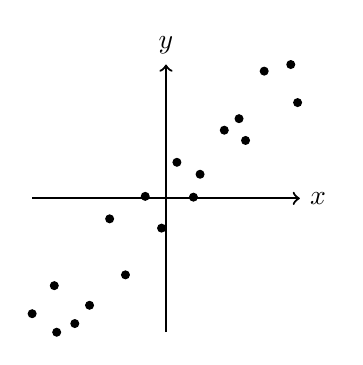
\begin{tikzpicture}
				\draw[->, thick] (-1.7,0)--(1.7,0) node[right]{$x$};
				\draw[->, thick] (0,-1.7)--(0,1.7) node[above]{$y$};
				\foreach \x in {-1.7,-1.5,...,1.7}{
					\pgfmathsetmacro\xcoord{\x+rand/10}
					\pgfmathsetmacro\ycoord{\x+rand/2}
					\pgfmathsetmacro\xcoord{\xcoord < -1.7 ? -1.7 : \xcoord}
					\pgfmathsetmacro\xcoord{\xcoord > 1.7 ? 1.7 : \xcoord}
					\pgfmathsetmacro\ycoord{\ycoord < -1.7 ? -1.7 : \ycoord}
					\pgfmathsetmacro\ycoord{\ycoord > 1.7 ? 1.7 : \ycoord}
					\node[circle,draw,fill=black,scale=0.3] at 
					(\xcoord,\ycoord) {};
				}
			\end{tikzpicture}
			\caption{a) Positive correlation.}
		\end{minipage}\hfill
		\begin{minipage}{0.32\textwidth}
			\centering
			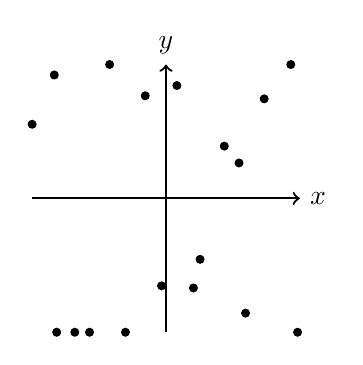
\begin{tikzpicture}
				\draw[->, thick] (-1.7,0)--(1.7,0) node[right]{$x$};
				\draw[->, thick] (0,-1.7)--(0,1.7) node[above]{$y$};
				\foreach \x in {-1.7,-1.5,...,1.7}{
					\pgfmathsetmacro\xcoord{\x+rand/10}
					\pgfmathsetmacro\ycoord{rand*2}
					\pgfmathsetmacro\xcoord{\xcoord < -1.7 ? -1.7 : \xcoord}
					\pgfmathsetmacro\xcoord{\xcoord > 1.7 ? 1.7 : \xcoord}
					\pgfmathsetmacro\ycoord{\ycoord < -1.7 ? -1.7 : \ycoord}
					\pgfmathsetmacro\ycoord{\ycoord > 1.7 ? 1.7 : \ycoord}
					\node[circle,draw,fill=black,scale=0.3] at 
					(\xcoord,\ycoord) {};
				}
			\end{tikzpicture}
			\caption{b) Uncorrelated/no correlation.}
		\end{minipage}\hfill
		\begin{minipage}{0.32\textwidth}
			\centering
			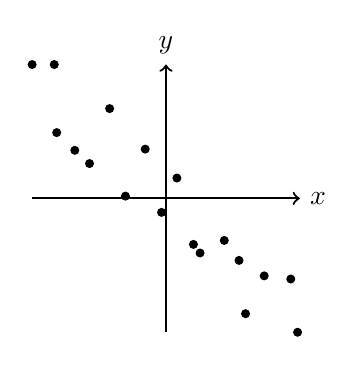
\begin{tikzpicture}
				\draw[->, thick] (-1.7,0)--(1.7,0) node[right]{$x$};
				\draw[->, thick] (0,-1.7)--(0,1.7) node[above]{$y$};
				\foreach \x in {-1.7,-1.5,...,1.7}{
					\pgfmathsetmacro\xcoord{\x+rand/10}
					\pgfmathsetmacro\ycoord{-\x+rand/2}
					\pgfmathsetmacro\xcoord{\xcoord < -1.7 ? -1.7 : \xcoord}
					\pgfmathsetmacro\xcoord{\xcoord > 1.7 ? 1.7 : \xcoord}
					\pgfmathsetmacro\ycoord{\ycoord < -1.7 ? -1.7 : \ycoord}
					\pgfmathsetmacro\ycoord{\ycoord > 1.7 ? 1.7 : \ycoord}
					\node[circle,draw,fill=black,scale=0.3] at 
					(\xcoord,\ycoord) {};
				}
			\end{tikzpicture}
			\caption{c) Negative correlation.}
		\end{minipage}\hfill
	\end{figure}
\end{frame}

\begin{frame}{Covariance of Numerical Data (I)}
	\begin{itemize}
		\item \textbf{\color{airforceblue}Covariance} \textbf{is similar to 
		correlation:}\\
		\begin{align}
			\text{Cov}(A,B) = 
			\frac{\sum_{i=1}^{n}(a_i-\overline{A})(b_i-\overline{B})}{N} 
		\end{align}
		\item \textbf{Pearson's correlation coefficient:}\\
		\begin{align}
			r_{A,B} = \frac{\sum_{i=1}^{N} 
			(a_i-\mu_A)(b_i-\mu_B)}{N\sigma_A\sigma_B} = 
			\frac{\sum_{i=1}^{N}(a_ib_i)-N\mu_A\mu_B}{N \sigma_A\sigma_B}, 
		\end{align}
		where $N$ is the number of tuples.
	\end{itemize}
\end{frame}

\begin{frame}{Covariance of Numerical Data (II)}
	\begin{itemize}
		\item \textbf{Positive covariance:}\\
		If $\text{Cov}(A,B) > 0$, then $A$ and $B$ tend to be either both 
		larger or both smaller than their expected values.
		\item \textbf{Negative covariance:}\\
		If $\text{Cov}(A,B) < 0$, then if $A$ is larger than its expected 
		value, $B$ is likely to be smaller than its expected value and vice 
		versa.
		\item \textbf{Independence:}
		\begin{itemize}
			\item $\text{Cov}(A,B) = 0$.
			\item \textbf{\color{airforceblue}But the converse is not true:} 
			Some pairs of random variables may have a covariance of $0$ but are 
			not independent. Only under some additional assumptions (e.g., the 
			data follow multivariate normal distributions) does a covariance of 
			$0$ imply independence.
		\end{itemize}
	\end{itemize}
\end{frame}

\begin{frame}{Covariance: An Example (I)}
	\begin{itemize}
		\item \textbf{Can be simplified in computation as:}
		\begin{align}
			\text{Cov}(A,B) & = E((A - E(A))(B-E(B)))            \\
			& = E(AB-AE(B)-E(A)B+E(A)E(B))       \\
			& = E(AB)-E(A)E(B)-E(A)E(B)+E(A)E(B) \\
			& = E(AB)-E(A)E(B).                  
		\end{align}
	\end{itemize}
\end{frame}

\begin{frame}{Covariance: An Example (II)}
	\begin{itemize}
		\item Suppose two stocks $A$ and $B$ have the following values within 
		some time:\\
		$(2,5), (3,8), (5,10), (4,11), (6,14).$
		\item If the stocks are affected by the same industry trends, will 
		their prices rise or fall together?
		\begin{align}
			E(A)            & = \frac{2+3+5+4+6}{5} = \frac{20}{5} = 
			4.                                               \\
			E(B)            & = \frac{5+8+10+11+14}{5} = \frac{48}{5} = 
			9.6.                                          \\
			\text{Cov}(A,B) & = \frac{2\cdot5 + 3\cdot 8 + 5 \cdot 10 + 4 \cdot 
			11 + 6 \cdot 14}{5} - 4\cdot 9.6 = 4. 
		\end{align}
		\item Thus, $A$ and $B$ rise together since $\text{Cov}(A,B) > 0$.
	\end{itemize}
\end{frame}